\subsection{Waveguides and Cavities \textbf{(L7)}}

 \subsubsection{\hyperref[Electromagnetic Crosswalk]{Electromagnetic Crosswalk}}
 
Imagine two electromagnetic beams intersecting at right angles. $(\bar{E_{H}},\bar{B_{H}})$ (moving in the horizontal direction) propagates in the $+x$ axis. $(\bar{E_{V}},\bar{B_{V}})$ (Vertical direction) propagates in the $+y$ direction. For simplicity, each beam is taken as a pure plane wave cut of transversely so its cross section is a perfect square of area $\lambda^{2}$ (Here $\lambda$ stands for the "space" each beam occupy). The fields are given by:
	
\begin{subequations}
\begin{align}
\vec{E}_{H} &= -E_{0} e^{i(kx - \omega t)} \hat{z}\\
c \vec{B}_{H} &= E_{0} e^{i(kx - \omega t)} \hat{y}\\
\vec{E}_{V} &= E_{0} e^{i(ky - \omega t)} \hat{z}\\
c \vec{B}_{V} &= E_{0} e^{i(ky - \omega t)} \hat{x}
\end{align}
\end{subequations}

\begin{figure}[h]
	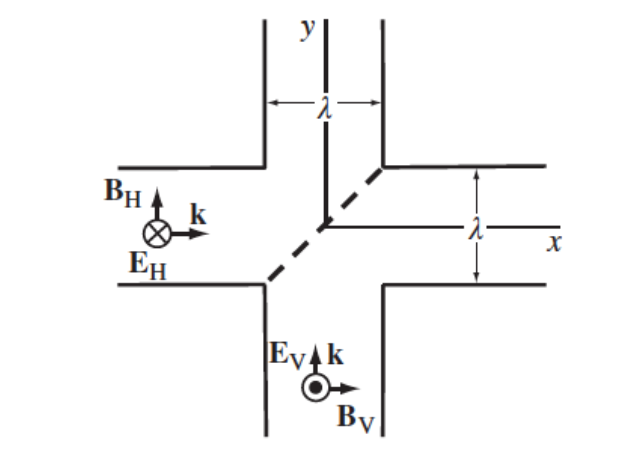
\includegraphics[width=8cm]{figures/crossbeams.png}
	\centering
	\caption{A sketch representation of the crossing beams and their components.}
\end{figure}

Where $\left|x\right|=\left|y\right|=\left|z\right|< \lambda/2$. The beams overlap in a cube centered at the origin where the total fields are given by a linear combination of vertical and horizontal ones.

\begin{enumerate}
	\item Calculate the time-averaged energy density $\langle u_{EM}(\bar{r})\rangle$ for the horizontal beam, the vertical beam and the total field in the overlap region. Show that the least of these takes its minimum value on the plane $x = y$. Compute $\bar{E}$ and $\bar{B}$ on this plane.
	\item Calculate the time-averaged Poynting vector $\langle S(\bar{r})\rangle$ for the H beam, the V beam and the total field as in previous part. Try to make a sketch of $\langle S(x,y)\rangle$ everywhere the fields are defined.
\end{enumerate}

\subsubsection{\hyperref[Waveguide Discontinuity]{Waveguide Discontinuity}}

Two rectangular waveguides with different major sides ($a_{1} < a_{2}$) along the $x$-axis and equal minor sides ($b_{1}= b_{2}$) along the $y$-axis\footnote{I rotate the axis in my solution, but the result should be the same.} are joined in the $z=0$ plane ($x=y=0$). The first region ($a_{1}$) propagates a $TE_{1,0}$ mode in the $+z$-direction towards the second region ($a_{2}$). Find the amplitude of some excited modes in the second region. Check also the limit where $a_{1} = a_{2}$\footnote{To find the modes and limits, consider that the remaining open space at $x=y=0$ between waveguides is closed by a perfect conductor, so modes cannot scape from our set up.}.

\subsubsection{\hyperref[Guess Who? (Wavefilter Edition)]{Guess Who? (Wavefilter Edition)}}

The figure below shows two circular conducting tubes in cross section. Each tube has a thin metal screen inserted at one point along its length. One screen takes the form of metal wires bent into concentric circles. The other takes the form of metal wires arranged like the spokes of a wheel. One of these tubes transmits only a low-frequency TE waveguide mode down the tube. The other transmits only a low-frequency TM waveguide mode down the tube. Explain which tube is which and why, using the fact that the fields of a general waveguide satisfy $\nabla \times \mathbf{E}_{\perp}=i \omega B_{z} \hat{z}$.

\begin{figure}[h]
	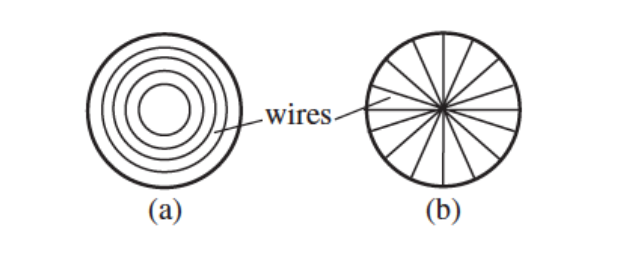
\includegraphics[width=8cm]{figures/2waveguides.png}
	\centering
	\caption{Both described wavefilters.}
\end{figure}

\subsubsection{\hyperref[An Electromagnetic Bat in a Resonant Cavity]{An Electromagnetic Bat in a Resonant Cavity}}

The two-dimensional vectors $\mathbf{k}_{m}$ shown below are inclined at angles $\theta_{m}=m \pi / 3$ with respect to the positive $x$ -axis. The vectors share a common magnitud $\left|\mathbf{k}_{m}\right|=k$.
Superpose six waves with alternating amplitudes to form the scalar function

\begin{equation}
	\psi(x, y, t)=\sum_{m=0}^{5}(-1)^{k} \sin \left(\mathbf{k}_{i} \cdot \mathbf{r}-c k t\right)
\end{equation}

Draw the outline of a two-dimensional resonant cavity which supports a TM mode built from $\psi(x, y, t)$.

\begin{figure}[h]
	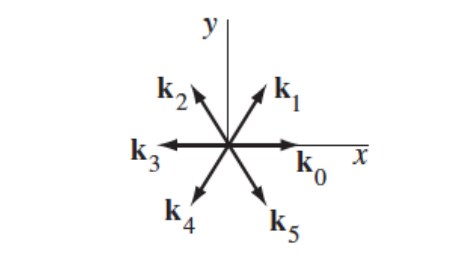
\includegraphics[width=8cm]{figures/6waves.png}
	\centering
	\caption{The vectorial distribution of the six waves.}
\end{figure}

\subsubsection{\hyperref[Cutting off the modes]{Cutting off the Modes}}

Transverse electric and magnetic waves are propagated along a hollow, right, circular cylinder with inner radius $R$ and conductivity $\sigma$. Find the cutoff frequencies of the various TE and TM modes. Determine numerically the lowest cutoff frequency (dominant mode) in terms of the tube radius and the ratio of cutoff frequencies of the next four higher modes to that of the dominant mode. For this part, assume that the conductivity of the cylinder is infinite.

\subsubsection{\hyperref[E: Rectangular Waveguide and its Modes]{E: Rectangular Waveguide and its Modes}}

Consider a waveguide whose section in the x-y plane is a rectangle with sides of length $a$ and $b$ (see figure). The waveguide walls are perfect conductors. The inside of the waveguide can be considered to be the vacuum.

\begin{figure}[h]
	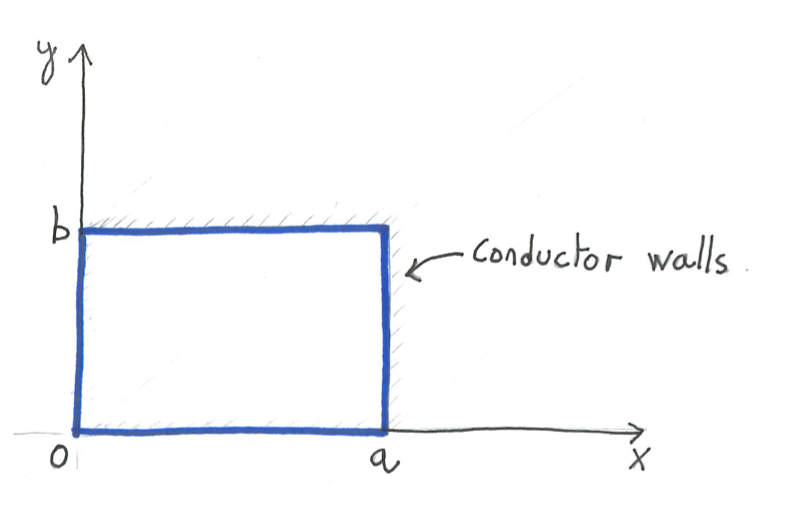
\includegraphics[width=8cm]{figures/examdec19p3.png}
	\centering
	\caption{A sketch picture of the waveguide's section.}
\end{figure}

\begin{enumerate}
	\item What are the boundary conditions that the electric $\vec{E}$ and magnetic $\vec{B}$ fields need to
	satisfy at the surface of a perfect conductor?
	\item Consider a function $\psi(x, y)$ that satisfies the equation
	
	\begin{equation}
		\left(\partial_{x}^{2}+\partial_{y}^{2}\right) \psi(x, y)+\gamma^{2} \psi(x, y)=0.
	\end{equation}

	in the interior of the rectangle for some $\gamma>0 .$ The cutoff frequencies of $T E$ and $T M$ modes for the waveguide are obtained determining the possible values of $\gamma>0$ in the equation above provided that the function $\psi(x, y)$ satisfies certain boundary conditions at the walls of the waveguide. For TM modes it must be that

	\begin{equation}
		\left.\psi\right|_{\text {wall }}=0,
	\end{equation}

	while for TE modes,

	\begin{equation}
		\left.\frac{\partial \psi}{\partial n}\right|_{\text {wall }}=0.
	\end{equation}

	Where $\left.\frac{\partial \psi}{\partial n}\right|_{\text {wall }}$ is the derivative in the direction perpendicular to the wall. The cutoff frequencies are then given by $\omega=c \gamma$.

	\begin{enumerate}
		\item For TM modes what is the smallest cut-off frequency?
		\item  For TE modes what is the smallest cut-toff frequency?
	\end{enumerate}

\end{enumerate}

\subsubsection{\hyperref[E: Mirror mirror on the wall...]{E: Mirror mirror on the wall...}}

Consider a waveguide whose section in the x-y plane is a square with sides of length $a$ (see figure A below). The waveguide walls are perfect conductors. The inside of the waveguide can be considered to be the vacuum.

\begin{figure}[h]
	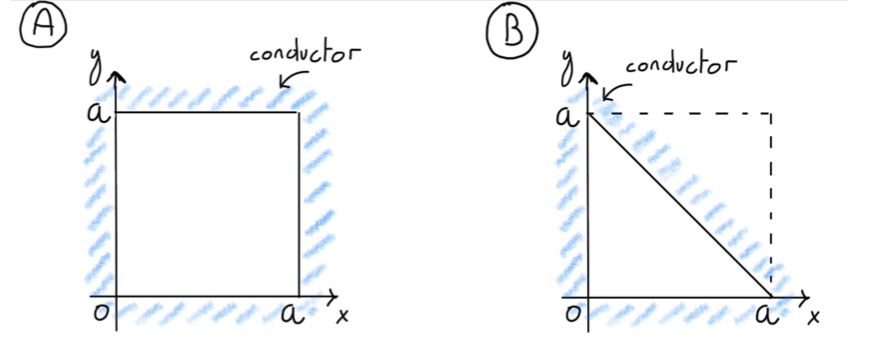
\includegraphics[width=12cm]{figures/examoct20p4.png}
	\centering
\end{figure}
\begin{enumerate}
	\item What are the boundary conditions that the electric $\vec{E}$ and magnetic $\vec{B}$ fields need to
	satisfy at the surface of a perfect conductor?
	\item Find the TM and TE modes for this wave-guide. For each mode display $\vec{E} \cdot \hat{z}$ for the TM modes and $\vec{B} \cdot \hat{z}$ for the TE modes. Also find the cutoff frequency for every mode.
	\item Certain distinct modes have the same cutoff frequency. Why? By taking appropriate linear combinations of the modes sharing the same cutoff frequency construct TM and TE modes for a waveguide whose section is a right isosceles triangle with catheti (short sides) of length $a$ (see figure B above). Show explicitly $\vec{E} \cdot \hat{z}$ for the TM modes and $\vec{B} \cdot \hat{z}$ for the TE modes.
\end{enumerate}

